\documentclass{article}
\usepackage{tikz}
\usetikzlibrary{positioning,arrows.meta}

\begin{document}

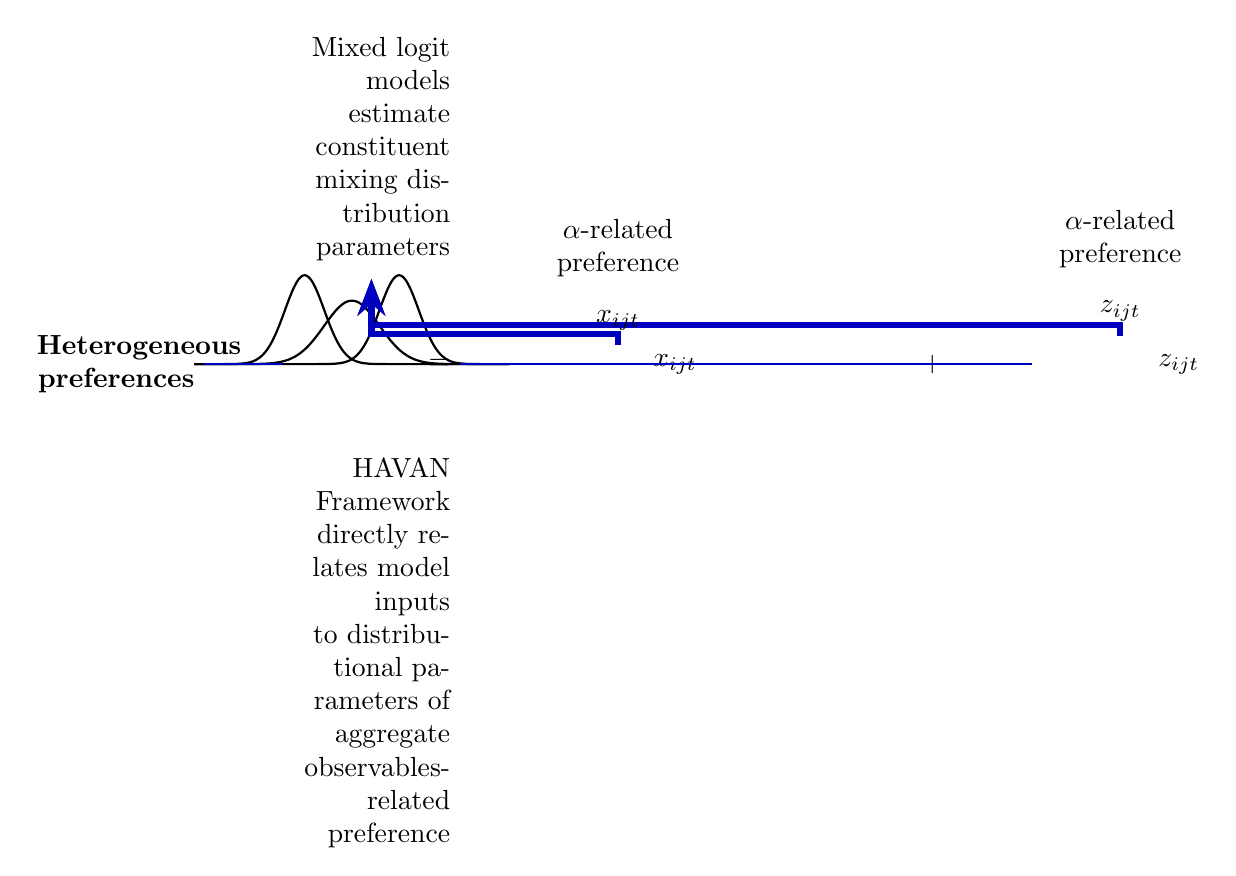
\begin{tikzpicture}[>=Stealth,
    declare function={gauss(\x,\m,\s)=1/(2*\s*sqrt(pi))*exp(-(\x-\m)^2/(2*\s^2));},
    every node/.style={text width=2cm, align=center},
    myarrow/.style={->, line width=0.8mm, draw=blue!75!black, shorten >=3pt, shorten <=3pt}]

\node [align=right] (hetero) at (-3,0) {\textbf{Heterogeneous \\ preferences}};
\node [align=right, right=of hetero] (eqn) {$=$};
\node [align=right, right=of eqn, inner sep=0] (xijt) {$x_{ijt}$};
\node [align=right, right=of xijt] (plus) {$+$};
\node [align=right, right=of plus] (zijt) {$z_{ijt}$};
\node [align=right, above=of eqn] (mix) {Mixed logit models estimate \\ constituent mixing distribution parameters};
\node [align=right, below=of eqn, inner sep=0] (havan) {HAVAN Framework directly relates model inputs \\ to distributional parameters of aggregate observables-related preference};

% Gaussian curve 1
\draw [domain=-2:2, samples=200, smooth, thick, color=black, variable=\x]
plot ({\x}, {gauss(\x,0,0.35)});
\fill [color=black, fill opacity=0.3] (-2,0) -- plot [smooth, tension=0.4] coordinates {(1,0) (2,0)} -- (2,0) -- cycle;

% Gaussian curve 2
\draw [domain=-2:2, samples=200, smooth, thick, color=black, variable=\x]
plot ({\x}, {gauss(\x,0.6,0.25)});
\fill [color=black, fill opacity=0.3] (0.6-0.05,0) -- plot [smooth, tension=0.4] coordinates {(0.6+0.05,0) (1.3,0)} -- (1.3,0) -- cycle;

% Gaussian curve 3
\draw [domain=-2:2, samples=200, smooth, thick, color=black, variable=\x]
plot ({\x}, {gauss(\x,-0.6,0.25)});
\fill [color=black, fill opacity=0.3] (-0.6-0.05,0) -- plot [smooth, tension=0.4] coordinates {(-0.6+0.05,0) (-1.3,0)} -- (-1.3,0) -- cycle;

% Connecting arrows
\draw [myarrow] (xijt.north) -- + (0,0.25) -| (mix);
\draw [myarrow] (zijt.north) -- + (0,0.25) -| (mix);

% Connecting lines
\draw [thick, color=blue!75!black] (hetero.east) -- (eqn.west);
\draw [thick, color=blue!75!black] (eqn.east) -- (xijt.west);
\draw [thick, color=blue!75!black] (eqn.east) -- (plus.west);
\draw [thick, color=blue!75!black] (eqn.east) -- (zijt.west);

% Labels for x and z
\node [above=5pt of xijt, anchor=south] (lab_xijt) {$x_{ijt}$};
\node [above=5pt of zijt, anchor=south] (lab_zijt) {$z_{ijt}$};

% Labels for Gaussian curves
\node [above=5pt of lab_xijt, anchor=south] {$\alpha$-related \\ preference};
\node [above=5pt of lab_zijt, anchor=south] {$\alpha$-related \\ preference};

\end{tikzpicture}

\end{document}